% ! TeX root = ../../master-thesis.tex

\section{Simulation}
\label{section:design:simulation}

The proposed approach for improving the observability and controllability of
the current simulator is to provide an interface on top of the base reactive
execution model of FRASP (Figure \ref{figure:simulation}). The design of this
interface abstracts from the underlying \ac{FRP} framework, specifically
Sodium, and from the approach adopted for managing the propagation of change in
the computational graph (e.g., concrete implementations may support
concurrency).

\begin{figure}[!ht]
  \centering
  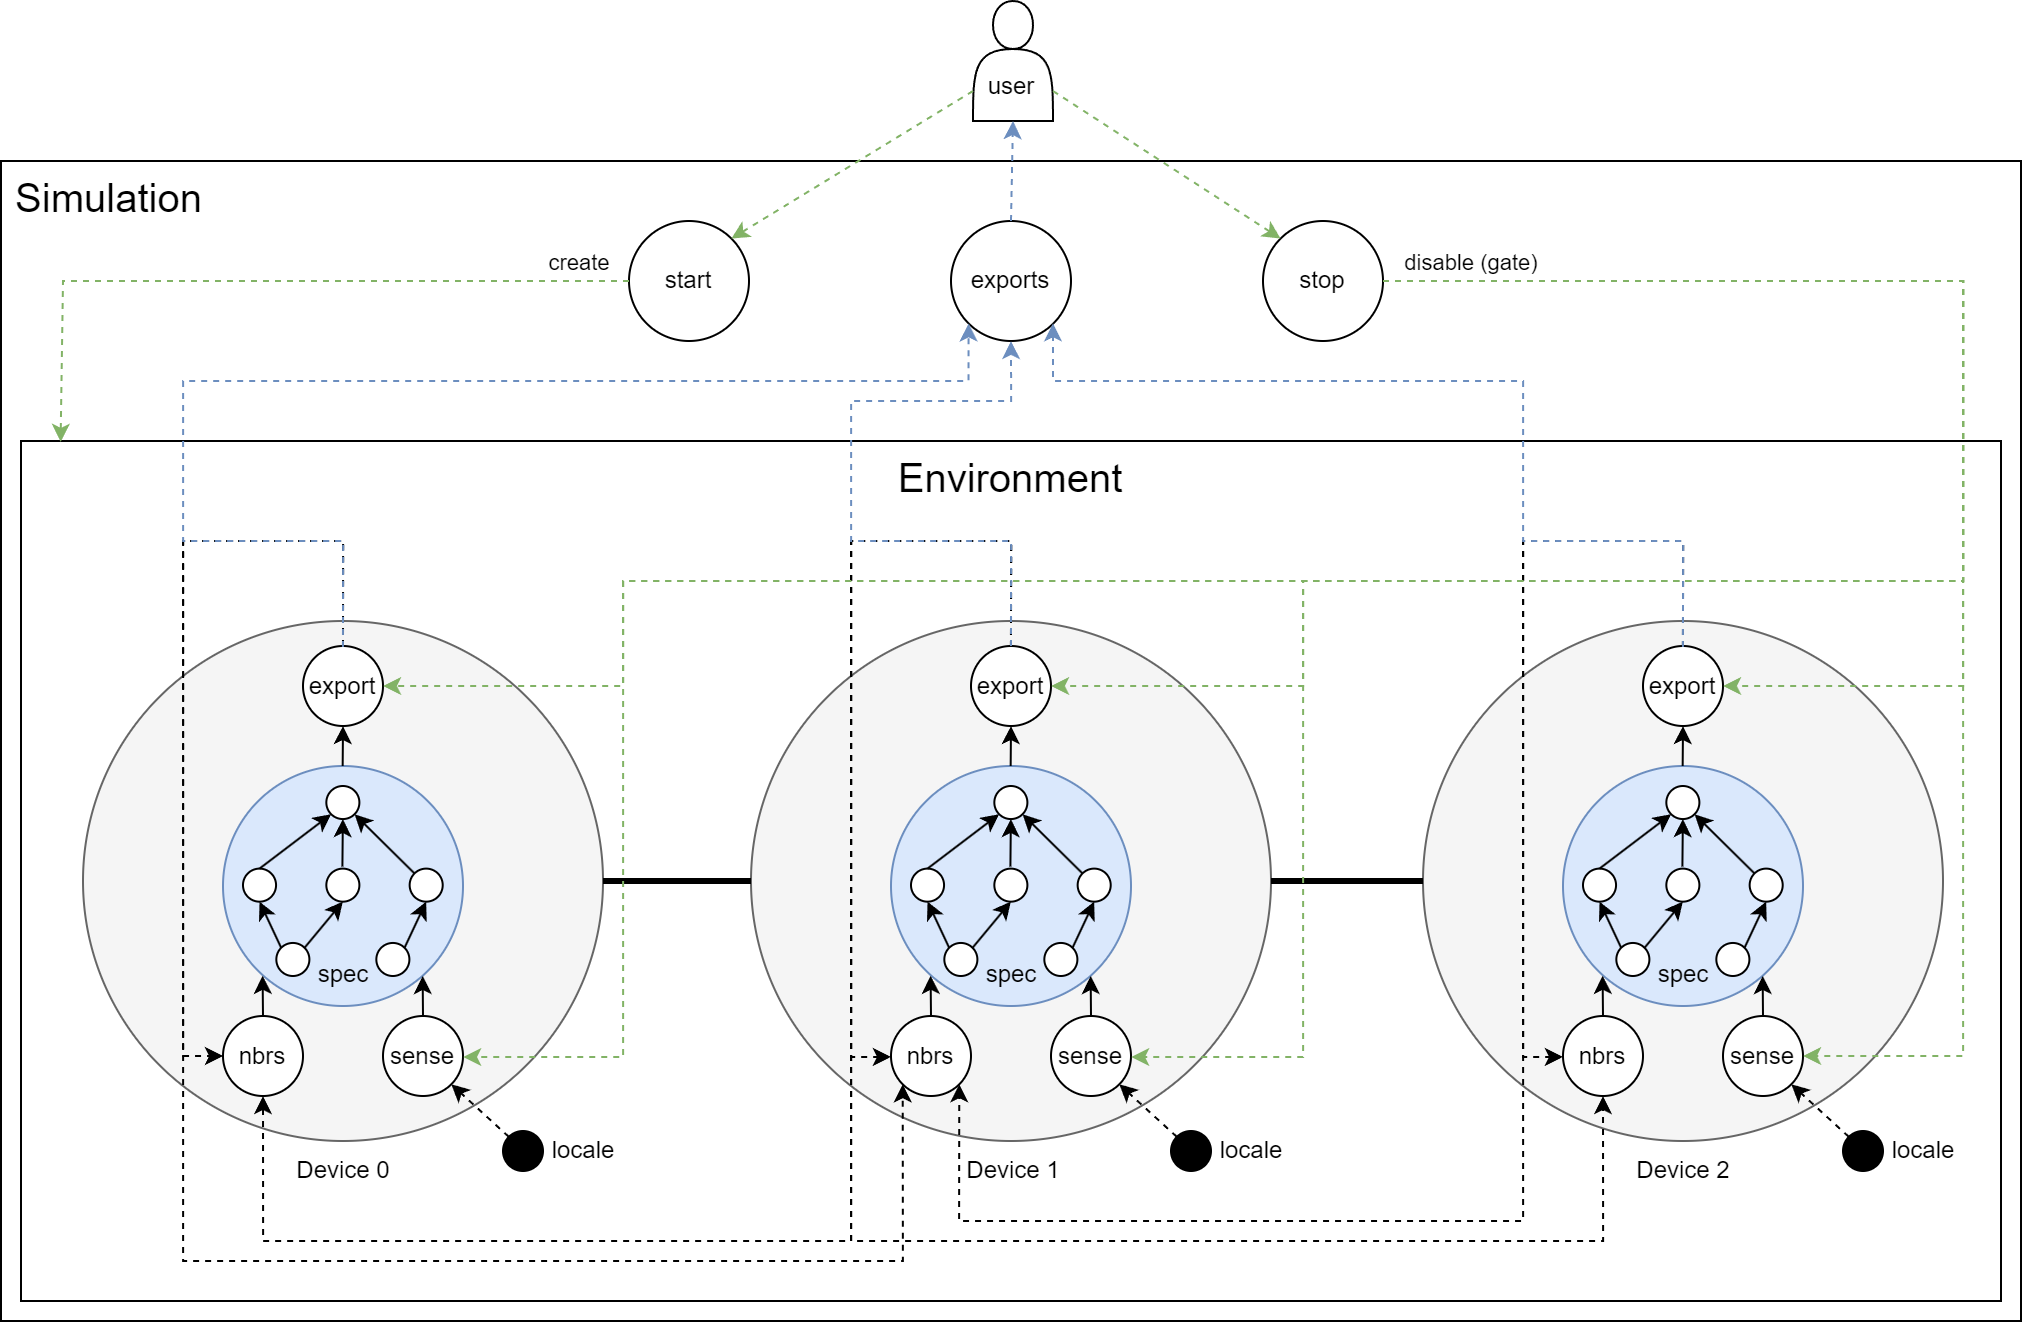
\includegraphics[width=1\textwidth]{resources/figures/simulation.png}
  \caption{
    The interface of a simulation for observing and controlling the
    underlying reactive execution model of FRASP. The user can now observe the
    state of a simulation (\texttt{exports}), start it (\texttt{start}) or stop
    it (\texttt{stop}). To support these new functionalities, new
    dependencies have been added for observability (\textit{blue dashed arrows})
    and controllability (\textit{green dashed arrows}).
  }
  \label{figure:simulation}
\end{figure}

Regarding observability, in static environments, the evolution of an aggregate
is uniquely described by its initial state and the sequence of device exports
(as discussed in Section \ref{section:analysis:aggregate-testing}). As a
consequence, complete observability of the evolution of an aggregate can be
achieved by simply collecting all the exports in the order they were produced,
whereas the initial state of the aggregate can be inferred from the
specification and environment provided during the configuration of the reactive
execution model (recall the configuration phase from Section
\ref{section:background:technologies:frasp}). In practice, the simulation
interface exposes a new reactive variable, called \texttt{exports}, derived by
\textit{merging} individual exports from each device. The firings of
\texttt{exports} can also be filtered, mapped and accumulated to provide
individual, regional or global views on the evolution of the aggregate.

Observability extends to dynamic environments by leveraging device sensors
(using the \texttt{sensor} and \texttt{nbrSensor} constructs) to reactively
produce exports containing changes in the environment.

Concerning controllability, the simulation interface offers a \texttt{start}
functionality, delaying the creation of the computational graph of the base
reactive execution model until requested by the user (instead of building the
graph when the simulation is created). This delay allows the user to declare
their own dependencies on the \texttt{exports} of the simulation before its
execution. As a consequence, forward referencing is required for
\texttt{exports} to declare its dependencies on the individual exports of the
devices.

To stop the simulation, it is possible to filter any future export when
requested by the user, freezing all views on the simulation (i.e.,
\texttt{exports}) and blocking any communication within the aggregate. However,
non-observable computation could still be triggered following a change in the
environment, even after the simulation is stopped. Therefore, to optimise the
simulation, any future percept of the device sensors should also be filtered
upon termination. Alternatively, the computational graph should be disposed of,
if possible.

An important aspect to consider for the observability of a simulation is
\textit{simulation time}, which measures the progress of a simulation. In
event-driven simulations, time is quantified as the number of events fired
since the beginning of the simulation (i.e., the number of firings of the
variable \texttt{exports}). Still, this representation has some implications,
such as time not advancing if no events are fired, affecting controllability.
Indeed, one cannot rely on the simulation time to stop the simulation without
prior knowledge about the evolution of the aggregate. For example, halting a
simulation after a specific number of events is unreliable, because one cannot
assume that the simulation will ever fire that many events, so the condition
may never be satisfied. However, a similar policy may be required to ensure
termination in aggregate tests, when the simulations never reach a stable
state, perhaps due to the nature of the specification or an unknown flaw in its
implementation.

Abstracting from the specific use case of halting the simulation, the problem
is that neither the user nor the simulation have an understanding of the
progress of the aggregate's evolution. On the one hand, the user lacks
information about the number of events that will be produced in the simulation,
which depends on the concrete implementations of the simulation and
specifications. On the other hand, the simulation lacks information about
possible changes of the environment, that may be triggered not only by the
device actuators, but also by external entities, such as the user. As a
consequence, none of the parties can evaluate when the evolution of the
aggregate should be considered concluded. This issue is referred to as the
\textbf{halting problem} in the following chapters.
